\documentclass[12pt,letterpaper]{article}
\usepackage[utf8]{inputenc}
\usepackage{amsmath,amsthm,amsfonts,amssymb,amscd}
\usepackage[table]{xcolor}
\usepackage[margin=2cm]{geometry}
\usepackage{graphicx}
\usepackage{multicol}
\usepackage{mathtools}
\usepackage[brazil]{babel}
\usepackage[default]{lato}
\usepackage[T1]{fontenc}
\usepackage{caption}
\usepackage{subcaption}
\newlength{\tabcont}
\setlength{\parindent}{0.0in}
\setlength{\parskip}{0.05in}

\DeclareMathOperator{\expv}{\mathbb{E}}
\DeclareMathOperator{\data}{\mathcal{D}}

\begin{document}
	
	\textbf{Nome}: Luís Felipe de Melo Costa Silva \\
	\textbf{Número USP}: 9297961 
	
	\begin{center}
		\LARGE \bf
		Lista de Exercícios 2 - MAC0460
	\end{center}
	
	\section*{Exercício 1}
		
	\textbf{a)} Vamos fazer $\mathbf{w}^\mathbf{T}(t) \cdot \mathbf{x}(t) = y^*(t)$. Como $\mathbf{x}(t)$ está classificado incorretamente, temos que os sinais de $y(t)$ e $y^*(t)$ são diferentes, ou seja, ou $y(t) = 1$ e $y^*(t) = -1$ ou $y(t) = -1$ e $y^*(t) = 1$. Portanto, $y(t) \cdot y^*(t)$ é sempre $-1$ e então, $y(t) \cdot y^*(t) < 0$ \\
		
	\textbf{b)} Usando (1.3):
	
	\begin{equation*}
		\begin{split}
			y(t)\mathbf{w}^\mathbf{T}(t+1)\mathbf{x}(t) & > y(t)\mathbf{w}^\mathbf{T}(t)\mathbf{x}(t) \\
			y(t)[\mathbf{w}^\mathbf{T}(t) + y(t)\mathbf{x}(t)]\mathbf{x}(t) & > y(t)\mathbf{w}^\mathbf{T}(t)\mathbf{x}(t) \\
			y(t)[\mathbf{w}^\mathbf{T}(t) + y(t)\mathbf{x}(t)]\mathbf{x}(t) & > y(t)\mathbf{w}^\mathbf{T}(t)\mathbf{x}(t) \\
			y(t)\mathbf{w}^\mathbf{T}(t)\mathbf{x}(t) + y(t)[y(t)\mathbf{x}(t)]\mathbf{x}(t) & > y(t)\mathbf{w}^\mathbf{T}(t)\mathbf{x}(t) \\
			y(t)\mathbf{w}^\mathbf{T}(t)\mathbf{x}(t) + y(t)[y(t)\mathbf{x}(t)]\mathbf{x}(t) & > y(t)\mathbf{w}^\mathbf{T}(t)\mathbf{x}(t) \\
			y(t)^2\mathbf{x}(t)^2 & > 0 
		\end{split}
	\end{equation*}

	\qed
	
	\textbf{c)} Quando temos uma classificação incorreta, temos que $y(t)\mathbf{w}^\mathbf{T}(t)\mathbf{x}(t) < 0$. A próxima atualização nos trará um valor $y(t)\mathbf{w}^\mathbf{T}(t+1)\mathbf{x}(t)$, que é maior do que o anterior, como provado no item acima. Isso nos deixa mais perto de um valor positivo, que é quando $\mathbf{x}(t)$ estará classificado corretamente.
 	
	\section*{Exercício 2}
	
	\textbf{a)} A hipótese $ h(\mathbf{x}) $ erra nos índices ímpares de $\mathbf{x}$, ou seja, em aproximadamente $ \frac{M}{2} $ índices. Logo, $ E_{\text{off}}(h,f) \cong \frac{1}{M}\cdot\frac{M}{2} \cong \frac{1}{2}$. \\
	
	\textbf{b)} Para cada $ \mathbf{x}_k, k \in \{1,..., N+M\}$, $ y $ pode assumir dois valores, $ -1 $ e $ +1 $, portanto, teremos $ 2^{N+M} $ funções distintas. Fixando um $N$, para garantir um conjunto $ \mathcal{D} $ sem ruídos, teremos $ 2^M $ funções distintas. \\
	
	\textbf{c)} O valor $ E_{\text{off}} = \frac{k}{M} $ mostra que temos $ k $ classificados incorretamente entre $ M $. O número de funções em que isso acontece é $ \binom{M}{k} $. \\
	
	\textbf{d)} Como o número de funções em que $ E_{\text{off}}(h,f) $ é $ \binom{M}{k} $, temos que: 
	
	\begin{equation*}
			\expv_f[E_{\text{off}}(h,f)] = \frac{1}{2^M} \sum_{k=0}^{M}\binom{M}{k} \cdot k = \frac{2^{M-1}M}{2^M} = \frac{M}{2}
	\end{equation*}
	
	\textbf{e)} No item anterior calculamos a esperança de $E_{\text{off}}$ em relação a $f$. O  que muda é a hipótese $ A(\mathcal{D}) $, e ela não influi no valor da esperança. Logo, a igualdade é válida.
	
	\section*{Exercício 3}
	
	\textbf{a)} Vamos minimizar $ E_{\text{in}}(h) $ com a derivada (achando o mínimo global).
	
	\begin{center} 
		$E'_{\text{in}}(h) = \sum_{n=1}^{N} 2(h-y_n) = 0$ \\
		$2Nh - \sum_{n=1}^{N} 2y_n = 0$ \\
		$Nh = \sum_{n=1}^{N} y_n$ \\
		$h = \frac{1}{N} \sum_{n=1}^{N} y_n$
	\end{center}
	
	\textbf{b)} A função módulo não é diferenciável. Por isso, para achar o ponto de mínimo, vamos quebrar nossa função em duas aqui. Para tal, seja um valor $ k $ tal que $ y_k \leq h \leq y+{k+1} $. Logo:
	
	\begin{center} 
		$E_{\text{in}}(h) = \sum_{n=1}^{k} (h-y_n) +  \sum_{n=k+1}^{N} (y_n-h) $\\
	\end{center}
	
	E então:
	
	\begin{center} 
		$E'_{\text{in}}(h) = \sum_{n=1}^{k} 1 +  \sum_{n=k+1}^{N} -1 = 0$\\
		$ \sum_{n=1}^{k} 1 = \sum_{n=k+1}^{N} 1 $\\
		$k = N-k$ \\
		$k = \frac{N}{2}$
	\end{center}
	
	\textbf{c)} O $E_{\text{in}}$ do primeiro item será bastante afetado, pois ele calcula a média, que tenderá a infinito, junto com $ \epsilon $. Já o $ E_\text{in} $ do segundo item não será afetado. Isso acontece pois ele utiliza a mediana, e ela é pouco ou nada afetada pelos \textit{outliers}.
	
	\section*{Exercício 4}
	
	Queremos que $\epsilon(M, N, \delta) = \sqrt{\frac{1}{2N} \text{ln} \frac{2M}{\delta}} \leq 0.05$. Teremos:
	
	\clearpage
	
	\begin{multicols}{2}
		\begin{equation*}
			\begin{split}
				\sqrt{\frac{1}{2N} \text{ln} \frac{2M}{\delta}} \leq 0.05 \\
				\frac{1}{2N} \text{ln} \frac{2M}{\delta} \leq 0.05^2 \\
				\frac{1}{2N} \leq \frac{0.05^2}{\text{ln} \frac{2M}{\delta}} \\
				2N \geq \frac{\text{ln} \frac{2M}{\delta}}{0.05^2} \\
				N \geq \frac{\text{ln} \frac{2M}{\delta}}{2 \cdot 0.05^2} \\
			\end{split}
		\end{equation*}
		
		Como $\delta = 0.03$: \\
		
		\textbf{a)} Para $M = 1$, $N \geq \frac{\text{ln} \frac{2}{0.03}}{2 \cdot 0.05^2} \cong 840$
		
		\textbf{b)} Para $M = 100$, $N \geq \frac{\text{ln} \frac{200}{0.03}}{2 \cdot 0.05^2} \cong 1761$
		
		\textbf{c)} Para $M = 10000$, $N \geq \frac{\text{ln} \frac{20000}{0.03}}{2 \cdot 0.05^2} \cong 2683$
	\end{multicols}
	
	
	\section*{Exercício 5}
	
	Do problema 2.5, temos que $ m_{\mathcal{H}}(N) \leq N^{d_{vc}} +1 $. Do problema 2.6, temos que $ m_{\mathcal{H}}(N) \leq \left(\frac{eN}{d_{vc}}\right)^{d_{vc}}$. 
	
	Portanto, teremos os seguintes gráficos:
	
	\begin{figure}[h]
		\centering
		\begin{subfigure}{.5\linewidth}
			\centering
			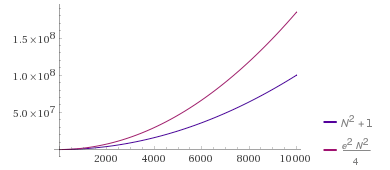
\includegraphics[width=\linewidth]{exercicio5a}
			\caption{$ d_{vc} = 2 $}
		\end{subfigure}%
		\begin{subfigure}{.5\linewidth}
			\centering
			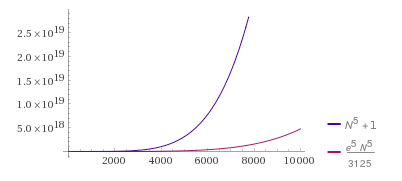
\includegraphics[width=\linewidth]{exercicio5b}
			\caption{$ d_{vc} = 5 $}
		\end{subfigure}
	\end{figure}
	
	Como queremos o limiar mais restritivo, quando $d_{vc} = 2$, o limite do Problema 2.5 é mais interessante. Analogamente, para $d_{vc} = 5$, o melhor é o do Problema 2.6.
	
	\section*{Exercício 6}
	
	Usando a fórmula (2.13) do livro, teremos:
	
	\begin{equation*}
		\begin{split}
			N & \geq \frac{8}{\epsilon^2} \cdot\text{ln}\left(\frac{4((2N)^{d_{vc}}+1)}{\delta}\right) \\
			& \geq \frac{8}{(0.05)^2} \cdot\text{ln}\left(\frac{4((2N)^{10}+1)}{0.05}\right) \\
			& \geq \frac{8}{0.025} \cdot\text{ln}\left(\frac{4((2N)^{10}+1)}{0.05}\right) \\
			& \geq 3200 \cdot\text{ln}(80((2N)^{10}+1)) \\
			& \geq 3200 \cdot\text{ln}(80((2N)^{10}+1)) \\
			& \geq 3200\cdot(\text{ln}80 + \text{ln}((2N)^{10}+1)) \\
			& \geq 14000 + 3200 \cdot\text{ln}((2N)^{10}+1))\\
			& \geq 14000 + 3200 \cdot\text{ln}((2N)^{10}) \\
			& \geq 14000 + 32000\cdot\text{ln}(2N) \\
			& \geq 14000 + 32000\cdot(\text{ln}(2) + \text{ln}(N)) \\
			& \geq 36000 + 32000 \cdot \text{ln}(N) \\ 
		\end{split}
	\end{equation*}
	
	Fazendo algumas estimativas, chegamos ao valor $ N \geq 453000 $.
	
	\section*{Exercício 7}
	
	Temos que $ y(x) = f(x) + \epsilon$, onde $ \epsilon $ é uma v.a. com $ \expv(\epsilon) = 0 $ e  var$(\epsilon) = \expv[\epsilon^2] = \sigma^2 $. Para auxiliar nos cálculos, vamos definir uma hipótese média $\bar{g}(x) = \expv_{\data}[g^{\data}(x)]$.
	
	\begin{equation*}
		\begin{split}
			\expv_{\data}[E_{out} (g^{(\data)})] & = \expv_{\data}[ \expv_{X,Y}[ (g^{(\data)}(x) - y(x))^2]] \\
			& = \expv_{X,Y}[ \expv_{\data}[ (g^{(\data)}(x) - y(x))^2]] \\
			& = \expv_{X,Y}[ \expv_{\data}[ (g^{(\data)}(x) -\bar{g}(x) + \bar{g}(x) - y(x))^2]] \\
			& = \expv_{X,Y}[ \expv_{\data}[ (g^{(\data)}(x) -\bar{g}(x))^2 + (\bar{g}(x) - y(x))^2 + 2 \cdot \overbrace{(g^{(\data)}(x) -\bar{g}(x))}^{0} \cdot (\bar{g}(x) - y(x))]] \\
			& = \expv_{X,Y}[ \expv_{\data}[ (g^{(\data)}(x) -\bar{g}(x))^2 + (\bar{g}(x) - y(x))^2]] \\
			& = \expv_{X,Y}[ \expv_{\data}[ (g^{(\data)}(x) -\bar{g}(x))^2] + \expv_{\data}[(\bar{g}(x) - y(x))^2]] \\
			& = \expv_{X,Y}[\expv_{\data}[ \text{var}(x) + (\bar{g}(x) - y(x))^2]] \\
			& = \text{var} + \expv_{X,Y}[(\bar{g}(x) - y(x))^2] \\
			& = \text{var} + \expv_{X,Y}[(\bar{g}(x) - f(x) - \epsilon)^2] \\
			& = \text{var} + \expv_{X,Y}[(\bar{g}(x))^2 + (f(x))^2 + \epsilon^2 - 2 \cdot \bar{g}(x) \cdot f(x) - 2 \cdot \bar{g}(x) \cdot \epsilon + 2 \cdot f(x) \cdot \epsilon] \\
			& = \text{var} + \expv_{X,Y}[(\bar{g}(x) - f(x))^2 + \epsilon^2 - 2 \cdot \bar{g}(x) \cdot \epsilon + 2 \cdot f(x) \cdot \epsilon] \\
			& = \text{var} + \expv_{X,Y}[\text{bias}(x)] + \expv_{X, Y} [\epsilon^2] - 2 \cdot \expv_{X, Y}[\bar{g}(x) \cdot \epsilon] + 2 \cdot \expv_{X,Y}[f(x) \cdot \epsilon] \\
			& \stackrel{ind.}{=} \text{var} + \text{bias } + \expv [\epsilon^2] - 2 \cdot \expv_X[\bar{g}(x)] \cdot \overbrace{\expv[\epsilon]}^{0} + 2 \cdot \expv_{X}[f(x)] \cdot \overbrace{\expv[\epsilon]}^{0} = \sigma^2 + \text{bias} + \text{var}
		\end{split}
	\end{equation*}
	
	\qed
	
	\section*{Exercício 8}
	
	\textbf{a)} Do enunciado, temos que o conjunto $\mathcal{H}$ possui funções no estilo $ ax+b $. Logo, usando a definição de $\bar{g}(x)$, e definindo como $K$ o número total de \textit{data sets}:
	
	\begin{equation*}
		\begin{split}
			\bar{g}(x) & = \expv_{\data}[g^{(\data)}(x)] = \expv_{\data}[a^{(\data)}\cdot x + b^{(\data)}] = \expv_{\data}[a^{(\data)}\cdot x] + \expv_{\data}[b^{(\data)}] \\
			& = \frac{1}{K} \sum_{k=1}^{K} a_k \cdot x + \frac{1}{K} \sum_{k=1}^{K} b_k = \frac{1}{K} \sum_{k=1}^{K} a_k \cdot x + b_k
		\end{split}
	\end{equation*}
	
	\textbf{b)} Fixando um número $ K $ de iterações, poderíamos fazer, a cada iteração:
	
	\begin{itemize}
		\item Gerar dois valores, $ x_1 $ e $ x_2 $, cada um retirado de uma distribuição Uniforme$ (-1, 1) $. Com isso, geramos dois pontos, usando a $ f(x) $, e temos nosso \textit{data set}.
		\item Rodar o algoritmo de aprendizado, que resultará em uma $ g(x) $.
	\end{itemize}
	
	Teremos $ K $ \textit{data sets} e $ K $ funções $ g(x) $. Com isso, podemos calcular:
	
	\begin{itemize}
		\item $ \bar{g}(x) $, com a média das $ g(x) $.
		\item O \textit{bias}, com o valor $ \expv_X[(\bar{g}(x) - f(x))^2] $.
		\item A \text{var}, fazendo $ \expv_X[\expv_{(\data)}(g^{\data}(x) - \bar{g}(x))^2]] $
		\item Por último, $ E_{out} $, com a fórmula $\expv_{\data}[E_{out} (g^{(\data)})] = \expv_{\data}[ \expv_X[ (g^{(\data)}(x) - f(x))^2]]$
	\end{itemize}
	
	\section*{Exercício 10}
	
	\textbf{a)} Vamos chamar de $ h(x) $ a saída do nosso algoritmo e $ C $ a variável que representa o custo. Teremos:
	
	\begin{itemize}
		\item cost(accept) = $\expv(C | h(x) = 1) = g(x) \cdot 0 + (1-g(x)) \cdot c_a = (1-g(x)) \cdot c_a$
		\item cost(reject) = $\expv(C | h(x) = -1) = g(x) \cdot c_r + (1-g(x)) \cdot 0 = g(x) \cdot c_r$
	\end{itemize}
	
	\textbf{b)} A regressão logística gera uma saída num intervalo contínuo $ [0,1] $. Quando usamos esse resultado para uma classificação binária, precisamos de um limiar $ \kappa $. O custo de aceite é igual ao custo de rejeite nesse ponto, já que o intervalo é contínuo. Então, fazendo $ g(x) = \kappa $, teremos:
	
	\begin{center}
		cost(reject) = cost(accept) \\
		$ (1-g(x)) \cdot c_a = g(x) \cdot c_r $ \\
		$ (1-\kappa) \cdot c_a = \kappa \cdot c_r $ \\
		$ c_a - \kappa \cdot c_a = \kappa \cdot c_r $ \\
		$ \kappa = \frac{c_a}{c_a + c_r} $
	\end{center}
	
	\qed
	
	\textbf{c)} Para o exemplo do supermercado, temos que $ c_a = 1 $ e $ c_r = 10 $. Portanto, teremos $ \kappa = \frac{1}{11} $, que indica um bom intervalo de aceite, já que é o falso negativo que incomoda. Já para a CIA, com $ c_a = 1000 $ e $ c_r = 1 $, $ \kappa = \frac{1000}{1001} $, e nos dá um intervalo bem restritivo para o aceite, de modo a evitar ao máximo falsos positivos.
	
\end{document}